\documentclass[handout]{beamer}
\usepackage[utf8]{inputenc}
\usepackage[T2A]{fontenc}
\usepackage[english]{babel}
\usepackage{graphicx}
\usepackage{array}
\usetheme{Warsaw}
\usecolortheme{wolverine}

\usepackage{fontawesome5}
\usepackage{listings}
\usepackage[all]{xy}
\usepackage{changepage}

\usepackage{tikz}
\usetikzlibrary{arrows.meta}

\definecolor{dkgreen}{rgb}{0,0.6,0}
\definecolor{gray}{rgb}{0.5,0.5,0.5}
\definecolor{mauve}{rgb}{0.58,0,0.82}

\definecolor{ukraine-blue}{rgb}{0,0.34,0.72}
\definecolor{ukraine-yellow}{rgb}{1,0.84,0}

\setbeamercolor{title}{fg=ukraine-blue,bg=ukraine-yellow}
\setbeamercolor{frametitle}{fg=ukraine-blue,bg=ukraine-yellow}
\setbeamercolor{section in head/foot}{fg=ukraine-blue}
\setbeamercolor{title in head/foot}{fg=ukraine-blue,bg=ukraine-yellow}
\setbeamercolor{author in head/foot}{fg=ukraine-yellow,bg=ukraine-blue}

\lstdefinelanguage{Haskell}%
  {otherkeywords={},%
   morekeywords={as,case,class,data,default,deriving,do,else,family,forall,foreign,hiding,if,import,in,infix,infixl,infixr,instance,let,mdo,module,newtype,of,proc,qualified,rec,then,type,where},%
   sensitive,%
   morecomment=[l]--,%
   morecomment=[n]{\{-}{-\}},%
   morestring=[b]"%
  }[keywords,comments,strings]%

\lstdefinelanguage{Cabal}%
  {otherkeywords={name,library,hs-source-dirs,exposed-modules,test-suite,main-is,build-depends,other-modules},%
   morekeywords={},%
   sensitive,%
   morecomment=[l]--,%
   morecomment=[n]{\{-}{-\}},%
   morestring=[b]"%
  }[keywords,comments,strings]%

\lstset{
  language=Haskell,
  showstringspaces=false,
  columns=flexible,
  keepspaces=true,
  basicstyle={\ttfamily},
  numbers=none,
  numberstyle=\tiny\color{gray},
  keywordstyle=\color{blue},
  commentstyle=\color{dkgreen},
  stringstyle=\color{mauve},
  escapeinside={<@}{@>},
  literate={²}{{$^2\;\!$}}1 {±}{{$\pm$}}1 {μ}{{$\mu$}}1 {α}{{$\alpha$}}1 {->}{{$\to$}}2 {=>}{{$\Rightarrow$}}2 {<-}{{$\leftarrow$}}2 {≤}{{$\leqslant$}}1 {<=}{{$\leqslant$}}1 {≥}{{$\geqslant$}}1 {>=}{{$\geqslant$}}1 {∷}{{$::$}}1 {::}{{$::$}}1 {...}{{\dots}}1
}

\def\ge{\geqslant}
\def\le{\leqslant}

\def\dd{\,.\,.\,}

\definecolor{darkblue}{rgb}{0,0,0.8}
\definecolor{darkgreen}{rgb}{0,0.6,0}
\definecolor{darkred}{rgb}{1,0,0}

\def\pros{\textcolor{darkgreen}{\bf Pros:} }
\def\cons{\textcolor{darkred}{\bf Cons:}\! }

\title[The \texttt{text} package: finally with UTF-8]{{The \texttt{text} package:} \\ finally with UTF-8}
\author[Andrew Lelechenko]{Andrew Lelechenko \\ \texttt{andrew.lelechenko@gmail.com}}
\institute{Barclays, London}
\date{ZuriHac, 12.06.2022}

\begin{document}

\begin{frame}
  \titlepage
\end{frame}

\begin{frame}[fragile]{String}

\begin{lstlisting}[language=Haskell]
type String = [Char]
\end{lstlisting}

\begin{itemize}
\item \pros supports full Unicode range, e. g., ``$\alpha\aleph\mathcal{A}$''.
\item \cons allocates two heap objects and 40 bytes per character.
\end{itemize}

\bigskip
\bigskip

\begin{figure}[c]
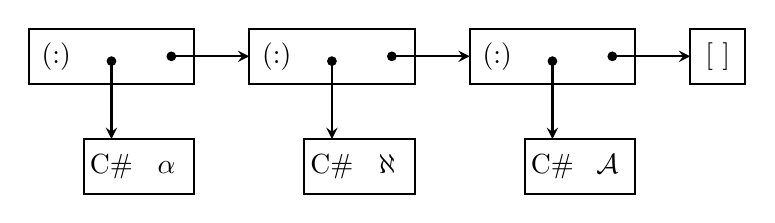
\begin{tikzpicture}[thick, scale=0.7]
\draw (0,3) rectangle (3,2);
\draw (4,3) rectangle (7,2);
\draw (8,3) rectangle (11,2);
\draw (12,3) rectangle (13,2);

\draw (1,0) rectangle (3,1);
\draw (5,0) rectangle (7,1);
\draw (9,0) rectangle (11,1);

\draw [{Circle[scale=0.7]}-stealth] (1.5,2.5) -- (1.5,1.0);
\draw [{Circle[scale=0.7]}-stealth] (5.5,2.5) -- (5.5,1.0);
\draw [{Circle[scale=0.7]}-stealth] (9.5,2.5) -- (9.5,1.0);

\draw [{Circle[scale=0.7]}-stealth] (2.5,2.5) -- (4.0,2.5);
\draw [{Circle[scale=0.7]}-stealth] (6.5,2.5) -- (8.0,2.5);
\draw [{Circle[scale=0.7]}-stealth] (10.5,2.5) -- (12.0,2.5);

\draw (0.5,2.5) node {(:)};
\draw (4.5,2.5) node {(:)};
\draw (8.5,2.5) node {(:)};
\draw (12.5,2.5) node {[ ]};

\draw (1.5,0.5) node {C\#};
\draw (2.5,0.5) node {$\alpha$\vphantom{\#}};

\draw (5.5,0.5) node {C\#};
\draw (6.5,0.5) node {$\aleph$\vphantom{\#}};

\draw (9.5,0.5) node {C\#};
\draw (10.5,0.5) node {$\mathcal{A}$\vphantom{\#}};

\end{tikzpicture}
\end{figure}

\end{frame}

\long\def\whatisascii{
\item ASCII assigns 128 code points, each encoded as 1 byte:
      newline, space, punctuation, digits, Latin letters.
\pause
\item Other 8-bit encodings extend ASCII
      up to 256 code points.
}

\begin{frame}[fragile]{ByteString}

\begin{lstlisting}[language=Haskell]
data ByteString = BS !(ForeignPtr Word8) -- payload
                     !Int                -- length

data ShortByteString = SBS ByteArray#
\end{lstlisting}

\begin{itemize}
\item \pros allocates a single heap object.
\item \pros spends 1 byte per character.
\item \cons does not support Unicode, only ASCII subset.
\end{itemize}

\bigskip
\bigskip

\pause

\begin{itemize}
\whatisascii
\end{itemize}

\end{frame}

\begin{frame}[fragile]{Encodings}

\begin{itemize}
\whatisascii
\pause
\item Unicode unifies multiple regional and national
      encodings into a~single character set.
\pause
\item 256 code points are not enough to fit the entire Unicode.
\pause
\item Well, surely, 64K ought to be enough for anybody!
\pause
\item Early Unicode embraced UCS-2 encoding, assigning up to 64K
      code points, each encoded as 2 bytes.
\pause
\item Guess what happened next?

\end{itemize}

\end{frame}

\begin{frame}{Unicode history}

\def\p{\phantom{0}}
\begin{table}[c]
\begin{tabular}{lrr@{~~~~}|@{~~~~}lrr}
Ver. & Date     & \#chars & Ver. & Date     & \#chars \\
\hline
1.0.0 & Oct 1991 &   7\,129 &  \p6.0 & Oct 2010 & 109\,384 \\
1.0.1 & Jun 1992 &  28\,327 &  \p6.1 & Jan 2012 & 110\,116 \\
1.1   & Jun 1993 &  34\,168 &  \p6.2 & Sep 2012 & 110\,117 \\
2.0   & Jul 1996 &  38\,885 &  \p6.3 & Sep 2013 & 110\,122 \\
2.1   & May 1998 &  38\,887 &  \p7.0 & Jun 2014 & 112\,956 \\
3.0   & Sep 1999 &  49\,194 &  \p8.0 & Jun 2015 & 120\,672 \\
3.1   & Mar 2001 &  \color{red}{94\,140} &  \p9.0 & Jun 2016 & 128\,172 \\
3.2   & Mar 2002 &  95\,156 &  10.0  & Jun 2017 & 136\,690 \\
4.0   & Apr 2003 &  96\,382 &  11.0  & Jun 2018 & 137\,374 \\
4.1   & Mar 2005 &  97\,655 &  12.0  & Mar 2019 & 137\,928 \\
5.0   & Jul 2006 &  99\,024 &  12.1  & May 2019 & 137\,929 \\
5.1   & Apr 2008 & 100\,648 &  13.0  & Mar 2020 & 143\,859 \\
5.2   & Oct 2009 & 107\,296 &  14.0  & Sep 2021 & 144\,697 \\
\end{tabular}
\end{table}

\end{frame}

\begin{frame}{UTF-32, UTF-16, UTF-8}

\begin{itemize}
\item UTF-32 aka UCS-4: each code point is encoded as 4 bytes:
  \begin{itemize}
  \item Fixed width encoding = trivial decoding.
  \item Incompatible both with ASCII and UCS-2.
  \end{itemize}
  \pause

\item UTF-16: the majority of code points are encoded as 2 bytes,
      but some
      as 4 bytes:
  \begin{itemize}
  \item Almost fixed width encoding = simple decoding.
  \item Compatible with UCS-2.
  \item Incompatible with ASCII.
  \end{itemize}
  \pause

\item UTF-8: ASCII code points are encoded as 1 byte,
      and others as 2, 3 or 4 bytes:
  \begin{itemize}
  \item Variable width encoding = complicated decoding.
  \item Compatible with ASCII.
  \end{itemize}

\end{itemize}

\end{frame}

\begin{frame}[fragile]{The {\tt text} package}

Developed by
  Thomas Harper
  (\href{https://www.cs.ox.ac.uk/files/3929/dissertation.pdf}{Fusion on Haskell Unicode Strings},
  MSc. Thesis, Oxford, 2008). The main goal was
  to ``create a~compact representation for Unicode strings that can take advantage
  of stream fusion''.

\medskip

\pause

\begin{block}{Ch. 4.1.4. Encoding shootout}
``\dots UTF-8, while more compact in many cases, pays for its complexity.
\dots Even though UTF-32 is faster
than UTF-16, sometimes much faster, its large footprint significantly reduces its usability. In
many cases, the distance between UTF-32 and UTF-16 is still far smaller than the gap between
UTF-16 and UTF-8, making it harder to justify doubling the space needed for a string''.
\end{block}

\medskip

\pause

The slowdown is correctly attributed to more complex branching
and worse branch prediction
for UTF-8 comparing to UTF-16.

\end{frame}

\begin{frame}[fragile]{Why migrate from UTF-16 to UTF-8?}

\begin{itemize}[<+->]
\item In 2011 Jasper Van der Jeugt submitted a GSoC proposal
      \href{https://jaspervdj.be/files/2011-gsoc-text-utf8-proposal.html}{``Convert the {\tt text} package to use UTF–8 internally''}.
\item The majority of the real world data is stored and transferred as UTF-8,
      because of the graceful degradation to ASCII.
\item Harper's benchmarks measured performance of {\tt text} transformations only
      {\em after} {\tt Text} was read and decoded from a~file
      and {\em before} it was written back.
\item For mostly-ASCII data UTF-8 takes almost 2x less memory than UTF-16.
\item The results, summarized by Jasper in
      \href{https://jaspervdj.be/posts/2011-08-19-text-utf8-the-aftermath.html}{``Text/UTF-8: Aftermath''},
      were inconclusive. The branch got abandoned and by 2021
      was $\sim800$ commits behind {\tt HEAD}.
\end{itemize}
\end{frame}

\long\def\utfchallenges{
\begin{frame}{UTF-8 challenges}

\begin{itemize}
\item Not every byte sequence is a valid UTF-8. In 2011 validation of UTF-8
      used to be almost as expensive as conversion to UTF-16.
      \pause
\item The fusion framework mandates that any materialized {\tt Text}
      is decoded into {\tt Stream Char} and encoded back,
      which is more expensive for UTF-8.
      \pause
\item Memory savings are less than 50\%, especially for short data:

\bigskip

\begin{figure}[c]
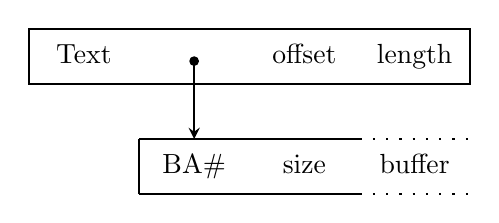
\begin{tikzpicture}[thick, scale=0.7]

\draw (0,2) rectangle (8,3);
\draw (1.0,2.5) node {Text\vphantom{g}};
\draw (5.0,2.5) node {offset\vphantom{g}};
\draw (7.0,2.5) node {length};

\draw [{Circle[scale=0.7]}-stealth] (3.0,2.5) -- (3.0,1.0);

\draw (2,0) -- (6,0);
\draw (2,1) -- (6,1);
\draw (2,0) -- (2,1);

\draw (3.0,0.5) node {BA\#};
\draw (5.0,0.5) node {size{\vphantom\#}};
\draw (7.0,0.5) node {buffer{\vphantom\#}};

\draw[loosely dotted] (6,0) -- (8,0);
\draw[loosely dotted] (6,1) -- (8,1);

\end{tikzpicture}
\end{figure}

\end{itemize}

\end{frame}
}

\utfchallenges

\begin{frame}{Five years later, 2016}

\begin{itemize}[<+->]
\item A renewed effort to migrate from UTF-16 to UTF-8 started in~2016,
      led primarily by Kubo Kov\'a\v{c}, Alexander Biehl and
      Herbert Valerio Riedel.
\item The authors rebased parts of Jasper's work in a bulk commit
      and continued from that point onward, accumulating $\sim100$~commits.
\item The work came to a halt in 2018 and by 2021
      was $\sim200$~commits behind {\tt HEAD}.
\item Benchmarks show severe regressions in certain disciplines.
\end{itemize}

\end{frame}

\begin{frame}{Emoji-driven development, 2021}

\begin{itemize}[<+->]
\item In March 2021 CLC revamped the team of {\tt text} maintainers.
\item Emily Pillmore and I submitted an HF proposal to migrate {\tt text}
      from UTF-16 to UTF-8, which was approved by the board in May 2021.
\item I started the implementation from the scratch
      and completed it by the end of August.
\item The pull request was reviewed and merged in September.
\item I prepared a series of release candidates in November,
      culminating with a release of {\tt text-2.0} on Christmas night.
      \bigskip
      \bigskip
\item What made the attempt \#3  more lucky?
\end{itemize}

\end{frame}

\begin{frame}{The most important principle}

\setbeamercolor{block body}{bg=ukraine-yellow}
\setlength{\textwidth}{1.05\textwidth}

\begin{block}{}
\bigskip
\centerline{\Huge\bf \color{ukraine-blue} ~ Invest in feedback loop! ~}
\bigskip
\end{block}

\end{frame}

\begin{frame}[fragile]{Unholy trick to avoid circular dependencies}

\begin{lstlisting}[language=Cabal]
name: text

library
  hs-source-dirs:  src
  exposed-modules: Data.Text

test-suite text-tests
  main-is:        Tests.hs
  hs-source-dirs: src tests
  build-depends:  base, test-framework
  -- but not text, because test-framework depends on it
  other-modules:  Data.Text
\end{lstlisting}

\end{frame}

\begin{frame}{Invest in feedback loop: tests}

\begin{itemize}
\item {\tt test-framework} is used to support GHC 7.0.
\pause
\item But it has plenty of dependencies and is not actively developed.
\pause
\item The closest replacement is {\tt tasty}.

\pause

\item
So I worked on {\tt tasty}
  \begin{itemize}
  \item to extend compatibility range back to GHC 7.0;
  \item to purge as many dependencies as possible.
  \end{itemize}

\pause

\item This succeeded, and now {\tt tasty} has the lowest dependency footprint
among Haskell testing frameworks.

\end{itemize}

\end{frame}

\begin{frame}{Invest in feedback loop: benchmarks}

\begin{itemize}[<+->]
\item Benchmarks are even worse: {\tt criterion} depends on {\tt text}
      transitively via multiple packages.
\item {\tt gauge} does not depend on {\tt text}, but often lags behind
      the most recent GHC.
\item We already have {\tt tasty}, which does not depend on {\tt text}.
      Can we upgrade it
      to become a benchmarking framework?
\item It appears {\tt tasty} has a modular architecture,
      and benchmarking can be implemented as a plugin.
\item I developed {\tt tasty-bench}:
  \begin{itemize}
  \item extremely lightweight and flexible,
  \item a drop-in replacement for {\tt criterion} and {\tt gauge},
  \item offers built-in comparison between runs and between
      benchmarks, invaluable for quick feedback.
  \end{itemize}
\end{itemize}

\end{frame}


\begin{frame}{Invest in CI heavily}

{\tt text} accumulated CI jobs for:

\begin{itemize}[<+->]
\item each supported version of GHC,
\item each build flag enabled and disabled,
\item Ubuntu, Windows, MacOS, FreeBSD, CentOS,
\item old Ubuntu releases,
\item i386, amd64, arm64, ppc64le, s390x,
\item IBM mainframes.
\end{itemize}

\end{frame}

\utfchallenges

\begin{frame}{Three engines for UTF-8 validation}

\begin{itemize}

\item {\tt simdutf} library.
  \begin{itemize}
  \item
    Daniel Lemire, Wojciech Mu\l{}a, Transcoding Billions
    of Unicode Characters per Second with SIMD instructions,
    Software: Practice and Experience, Sep 2021.
  \item
    Implemented in C++, hard to link from Haskell.
  \item
    Returns a boolean flag.
  \end{itemize}
  \pause

\item {\tt isValidUtf8} function.
  \begin{itemize}
  \item Developed by Koz Ross, in-kind donation from MLabs to HF.
  \item Implemented in C, a part of {\tt bytestring-0.11.2.0}.
  \item Returns a boolean flag.
  \end{itemize}
  \pause

\item Native state machine.
  \begin{itemize}
  \item Adapted from earlier UTF-8 decoding routine in C.
  \item Translated to Haskell.
  \item Returns a state of decoder.
  \item Suitable for malformed and partial data.
  \end{itemize}

\end{itemize}

\end{frame}

\begin{frame}[fragile]{Fusion of {\tt Text}}

\begin{itemize}[<+->]
\item Text has two equivalent representations:
  as a materialized buffer {\tt Text} and as a {\tt Stream} of {\tt Char}s.
\item Some functions have two versions: one for {\tt Text}
  and one for {\tt Stream Char}.
\item But most were implemented as wrappers:

\begin{lstlisting}[language=Haskell]
foo :: Text -> Text
foo = unstream . fooS . stream

stream :: Text -> Stream Char
unstream :: Stream Char -> Text
fooS :: Stream Char -> Stream Char
\end{lstlisting}

\item Each fused transformation pipeline needed to decode and encode UTF-8 at least once.
\end{itemize}

\end{frame}

\begin{frame}[fragile]{Tale of two tails}

{\tt tail} takes $O(1)$ time, but {\tt tail} . {\tt tail} takes $O(n)$ time.

\pause

\begin{lstlisting}[language=Haskell]
tail :: Text -> Text
tail (Text arr off len) =
  Text arr (off + delta) (len - delta)
    where
      delta = iter_ t 0

{-# RULES
  "fuse tail" [~1] tail = unstream . S.tail . stream
  "unfuse tail" [1] unstream . S.tail . stream = tail
  "fusion" stream . unstream = id
  #-}
\end{lstlisting}

\pause

So {\tt tail} remains {\tt tail} after optimizations,
but {\tt tail} . {\tt tail} becomes
{\tt unstream} . {\tt S.tail} . {\tt S.tail} . {\tt stream},
decoding everything in full.

\end{frame}

\begin{frame}[fragile]{No implicit fusion}

\begin{itemize}[<+->]
\item Long pipelines
      of {\tt Text} transformations are rare and unlikely to bottleneck because
      of lack of fusion alone.
\item Instead we need to focus on slicing and concatenation,
      which are precisely where uncontrolled implicit fusion is harmful.
\item Let's disable implicit fusion and rewrite
      every function to operate on buffers directly.
\item I spend
  \begin{itemize}
  \item one night implementing a full switch from UTF-16 to UTF-8,
  \item and three months
      rewriting routines to avoid streaming.
  \end{itemize}
\end{itemize}

\end{frame}

\begin{frame}{Performance after transition to UTF-8}

\begin{itemize}
\item {\tt decodeUtf8} is up to 10x faster for non-ASCII texts.
\pause
\item {\tt encodeUtf8} is 1.5--4x faster for strict, 10x faster for lazy Text.
\pause
\item {\tt take} / {\tt drop} / {\tt length} are up to 20x faster.
\pause
\item {\tt toUpper} / {\tt toLower} are 10-30\% faster.
\pause
\item {\tt Ord} instance is typically 30\%+ faster.
\pause
\item {\tt isInfixOf} and search routines are up to 10x faster.
\pause
\item {\tt replicate} of {\tt Char} is up to 20x faster.
\end{itemize}

\bigskip
\pause

Geometric mean of relative benchmark times is 0.33
\par \hfill = an average benchmark is 3x faster.

\end{frame}

\begin{frame}[fragile]{Migration efforts}

Multiple libraries rely on the internal representation of {\tt Text}:

\begin{itemize}
\item {\tt attoparsec} reuses parts of {\tt Text} to store auxiliary data.
\pause
\item Streaming libraries often contain C code for UTF-8 decoding.
\pause
\item {\tt aeson} uses C code to unescape JSON UTF-8 strings
      and store them as UTF-16 in one go.
\pause
\item LSP positions assume UTF-16, impacting HLS.
\pause
\item {\tt text-icu} communicates to {\tt libicu}, which uses UTF-16.
\end{itemize}

\bigskip
\pause

Huge thanks to all maintainers involved in the migration!
\pause

\begin{itemize}
\item All Stackage Nightly packages are compatible with {\tt text-2.0}.
\pause
\item {\tt text-2.0} will be shipped with GHC 9.4.
\end{itemize}

\end{frame}


\begin{frame}[fragile]

\begin{itemize}
\item {\tt text-2.0} is ready for the prime time, give it a try today!
\pause
\item We are looking for new contributors, feel free to get in touch.
\pause
\item A brand new {\tt text-builder-linear} is out, up to 20x faster.
\end{itemize}
\pause


\bigskip

\setbeamercolor{block body}{bg=ukraine-yellow}

\begin{block}{}
\bigskip
\centerline{\Huge\bf \color{ukraine-blue} Thank you!}
\bigskip
\end{block}

\bigskip
\bigskip
\bigskip

\centerline{\color{ukraine-blue}
\faAt\ andrew.lelechenko@gmail.com ~~ \par \faTelegram\ Bodigrim
\hspace{27mm}
}

\medskip

\centerline{\color{ukraine-blue}
\hspace{15mm}
\faGithub\ github.com/haskell/text ~~
\faGithub\ github.com/Bodigrim/my-talks
}

\end{frame}

\end{document}
